\documentclass[11pt]{article}
\usepackage{times}
\usepackage{url}
\usepackage{latexsym}
\usepackage{graphicx}
% För svenska tecken åäö
\usepackage[T1]{fontenc}
\usepackage[utf8]{inputenc}
\usepackage{tabularx}
\usepackage[margin=3.4cm]{geometry}
\usepackage{titlesec}
\usepackage{csquotes}
% Created by Hercules Dalianis, December 24, 2019

\usepackage[square,sort,comma,numbers]{natbib}
\usepackage{hyperref} 
%\bibliographystyle{apalike}
\bibliographystyle{vancouver}

% square brackets and comma separator between authors
\setcitestyle{square,comma}

\usepackage{authblk}

\usepackage{abstract}

\title{Title of Your HealTAC Paper Submission}
\begin{document}

\renewcommand\Authand{}

\author[1]{Firstname A. Lastname}
\author[2]{ Firstname B. Lastname}

\affil[1]{Institution, City, State, Country}
\affil[2]{Institution, City, State, Country}
 
\date{}
\maketitle

% Vänsterjustera abstract heading
\renewcommand{\absnamepos}{flushleft}
\setlength{\absleftindent}{0pt}
\setlength{\absrightindent}{0pt}

\section*{Introduction}
This section should be used as a starting point for your extended abstract. Explain why this research or implementation is important, interesting and/or needed. Begin by describing the problem or situation that motivates the research. Briefly refer to the current state of research in the field and specify a “gap” or problem you will address as the key objective(s) of your contribution. If the study has hypotheses, mention them here.
All the sections mentioned here are compulsory (Introduction, Methods/Data, Results, Conclusion, Study Context, References). Each extended abstract submission should be up to 2 pages, inclusive of all sections (for other submissions, see below). Prepare your submissions according to the format and presentation requirements described here. Use a single-column formatting (Arial, at least 10pt). Extended abstract can include references. Follow the Vancouver Style (see: \href{https://www.icmje.org/index.html}{www.icmje.org/index.html}) - for example, this sentence has two reference citations \citep{ta1983gardner,gardner1990computer}.


\begin{figure}[h]
\centering
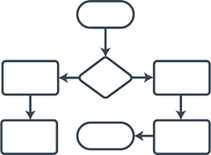
\includegraphics[width=0.5\linewidth]{template-image.png}
\caption{A diagram.}
\label{template-image}
\end{figure}



\section{Methods and Data}
Use this section to explain how you have conducted your study. Include information about your data, methods, implementation, and evaluation. Provide enough information for the reader to be able to understand how the study was conducted, how the data were collected, annotated and/or analysed, and whether these choices were sensible. 
You can include additional figures to describe the workflow or data. Figures (see Figure \ref{template-image}) need to be referenced from text and placed as close to the corresponding text as possible and not extend beyond one page. Make sure all tables and figures are labeled and numbered separately.

\section{Results}
In this section, present your findings and evaluation, referring to your main objectives and questions. While the Results section typically contains only the findings, you can include here some explanation and discussion as well. Use tables and figures as appropriate. Note that captions go above tables (see Table 1) and beneath figures. 

\begin{table}[h!]

\caption{Submission type, abstract length, and page length maximum.}
\label{sub-type}
\begin{tabular}{ |p{6cm}|p{8cm}| } 
 \hline
 \textbf{Submission type} & \textbf{Page Length Maximum and structure}  \\ 
 \hline
Extended abstract  & 2 pages; use this template \\
 \hline
 PhD and fellowship project description & 4 pages; use this template \\
 \hline
 Panel proposal & 2 pages; use the following sections: Introduction, Session aim and design, Speakers, Expected audience. \\
 \hline
 Software demo session & 2 pages; use this template and adjust as appropriate \\
 \hline
\end{tabular}
\end{table}


\section{Conclusion}
Summarise your main findings, map them to your objectives and connect them to other research. You can also discuss limitations of your study, and use these limitations as reasons to suggest additional, future research.

\section{Study context}
Provide additional information about the context of this study, including any ethics consideration and approvals, funding, stakeholder involvement (e.g. patients and public), availability of data and methods, conflicts of interest, collaborators, etc.


\bibliography{template-references.bib}
\end{document}
